\documentclass[12pt, twoside]{article}
\usepackage[letterpaper, margin=1in, headsep=0.5in]{geometry}
\usepackage[english]{babel}
\usepackage[utf8]{inputenc}
\usepackage{amsmath}
\usepackage{amsfonts}
\usepackage{amssymb}
\usepackage{tikz}
\usetikzlibrary{quotes, angles}
\usepackage{graphicx}
\usepackage{enumitem}
\usepackage{multicol}

\newif\ifmeta
\metatrue %print standards and topics tags

\title{Regents Geometry}
\author{Chris Huson}
\date{September 2020}

\usepackage{fancyhdr}
\pagestyle{fancy}
\fancyhf{}
\renewcommand{\headrulewidth}{0pt} % disable the underline of the header
\raggedbottom


\fancyhead[LE]{\thepage}
\fancyhead[RO]{\thepage \\ Name: \hspace{4cm} \,\\}
\fancyhead[L]{BECA / Dr. Huson / Geometry 06-Analytic-geometry\\* pset ID: 74}

\begin{document}

\subsubsection*{6-10bDN-Graphing}
\begin{enumerate}
\item Checklist:
  \begin{itemize}
    \item[$\square$]   I used a straight edge to make the lines
    \item[$\square$]   I labeled each line with its original equation
    \item[$\square$]   I labeled the intersection as an ordered pair
    \item[$\square$]   I answered the question, explained, and wrote down the two slopes
  \end{itemize}
  Graph and label the two equations. Mark their intersection as an ordered pair.
    \begin{multicols}{2}
      $y =\frac{2}{3}x+1$ \\
      $y=\frac{2}{3}x-4$
    \end{multicols}     \vspace{0.1cm}
    Are the lines parallel, perpendicular, or neither? Justify your answer.
    \vspace{2.5cm}

    \begin{center} %4 quadrant regents grid w T-Chart
    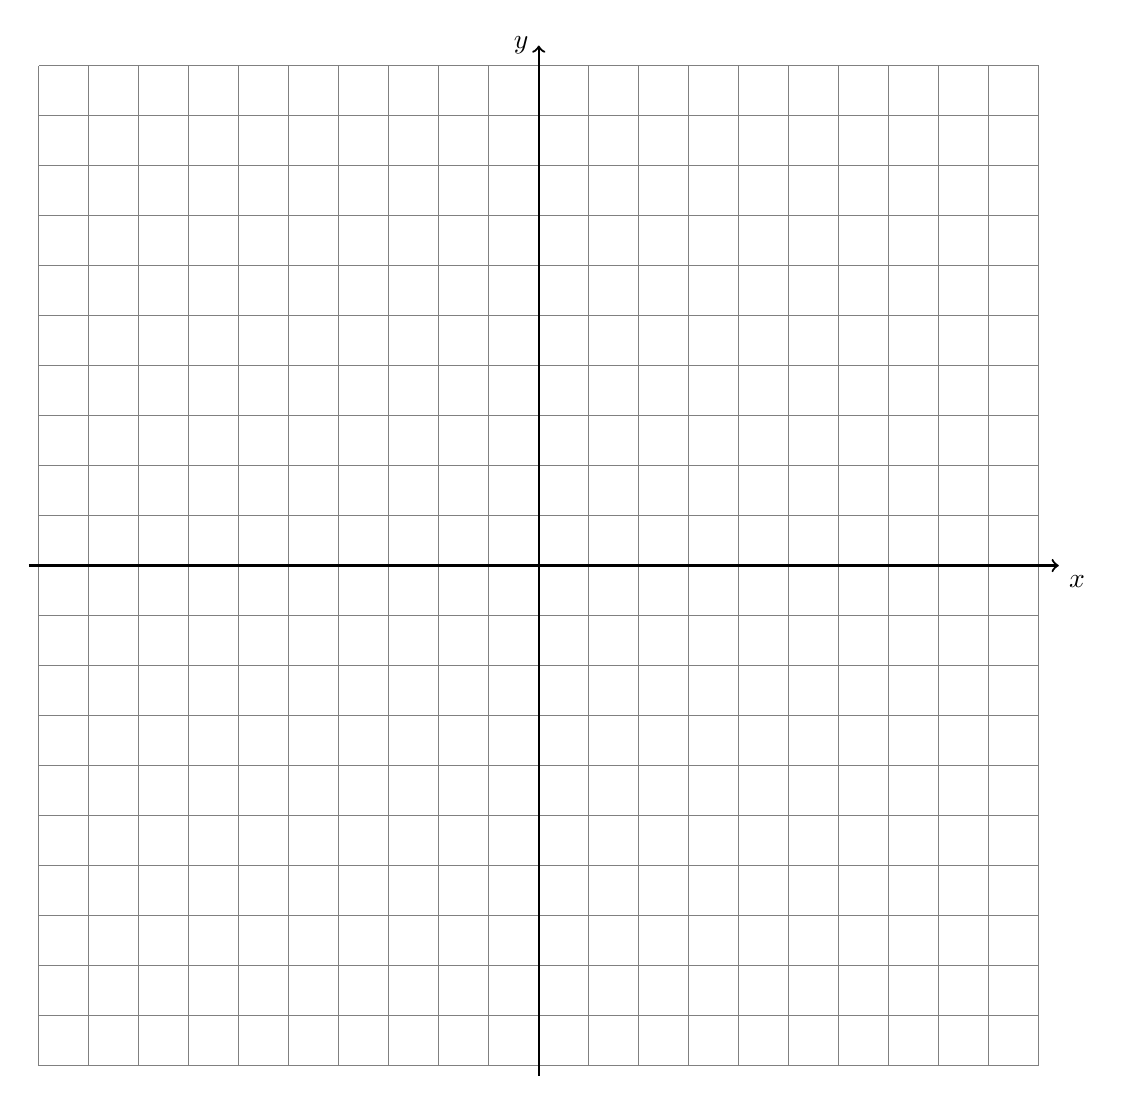
\begin{tikzpicture}[scale=.635]
      \draw [help lines] (-10,-10) grid (10,10);
      \draw [thick, ->] (-10.2,0) -- (10.4,0) node [below right] {$x$};
      \draw [thick, ->] (0,-10.2)--(0,10.4) node [left] {$y$};
    \end{tikzpicture}
    \end{center}

\newpage
\item Graph and label the two equations. Mark their intersection as an ordered pair.
      \begin{multicols}{2}
        $y =\frac{1}{2}x+3$ \\[0.25cm]
        $y=-2x+8$ \\
        Are the lines parallel, perpendicular, or neither? Justify your answer.
      \end{multicols}     \vspace{0.1cm}
      %Are the lines parallel, perpendicular, or neither? Justify your answer.
      \vspace{1cm}

      \begin{flushright} %4 quadrant regents grid w T-Chart
      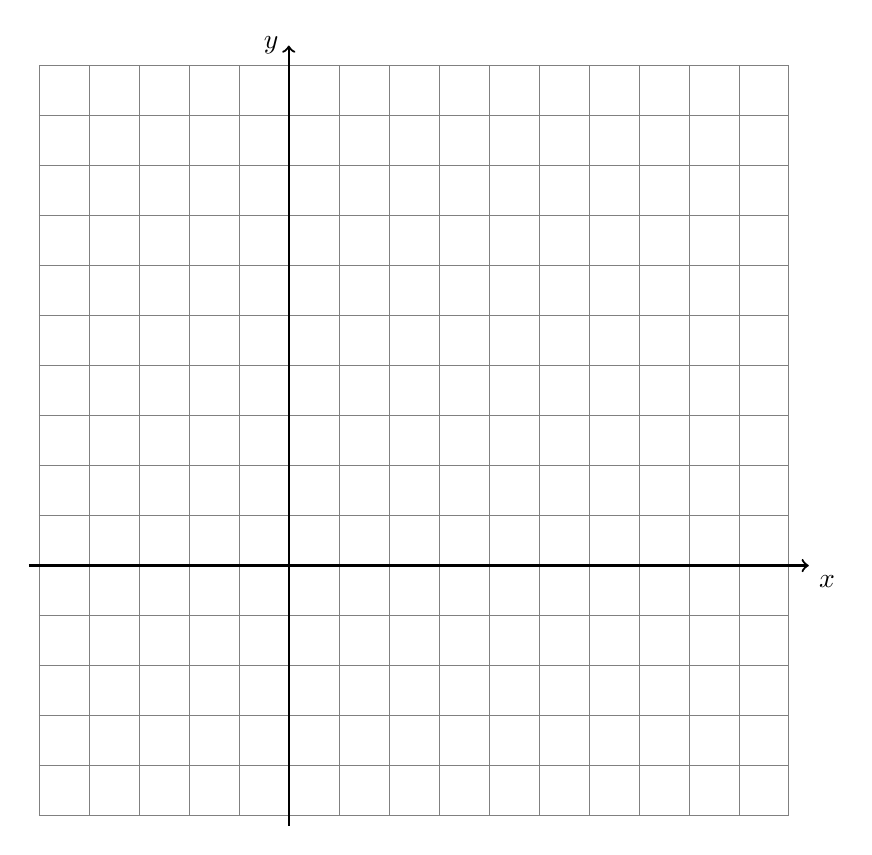
\begin{tikzpicture}[scale=.635]
        \draw [help lines] (-5,-5) grid (10,10);
        \draw [thick, ->] (-5.2,0) -- (10.4,0) node [below right] {$x$};
        \draw [thick, ->] (0,-5.2)--(0,10.4) node [left] {$y$};
      \end{tikzpicture}
      \end{flushright}

\item Apply a dilation mapping $\triangle ABC \rightarrow \triangle A'B'C'$ with a factor of $k=2$ on the grid, labeling the image.

    \begin{flushright} %4 quadrant regents grid w T-Chart
    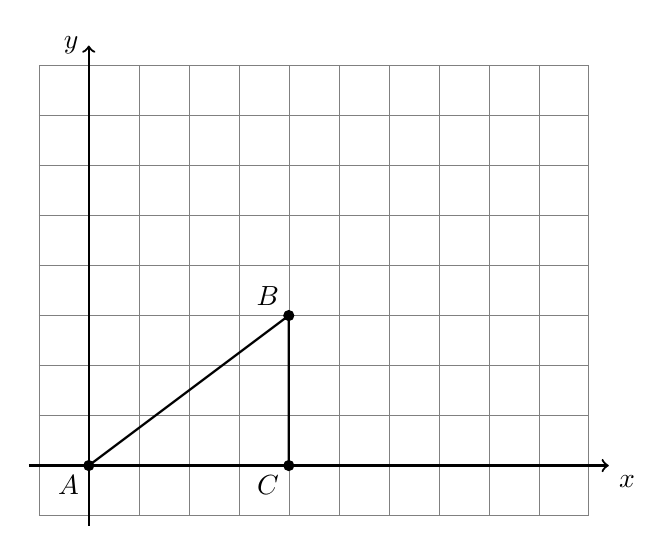
\begin{tikzpicture}[scale=.635]
      \draw [help lines] (-1,-1) grid (10,8);
      \draw [thick, ->] (-1.2,0) -- (10.4,0) node [below right] {$x$};
      \draw [thick, ->] (0,-1.2)--(0,8.4) node [left] {$y$};
      \draw [thick] (0,0)--(4,0)--(4,3)--cycle;
      \draw [fill] (0,0) circle [radius=0.1]node[below left]{$A$};
      \draw [fill] (4,0) circle [radius=0.1]node[below left]{$C$};
      \draw [fill] (4,3) circle [radius=0.1]node[above left]{$B$};
    \end{tikzpicture}
    \end{flushright}

\end{enumerate}
\end{document}